\section{Visual Darkroom}
\label{appendix:visual_gridworld}
We adapted the Darkroom environment to produce high-dimensional visual observations to demonstrate Headless-AD's capability to generalize to new action spaces in more complex settings. In this modified version, the grid is visually represented, with the agent's position indicated in red (see \Cref{fig:visual_gridworld_img}). This change introduces a more complex observation space. For the model to handle these high-dimensional visual observations, we integrated a convolutional network that converts the visual input into an embedding of size 'token\_dim'.

\begin{figure*}[h]
    \vskip 0.2in
    \centering
    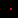
\includegraphics[width=0.2\textwidth]{images/visual_gridworld_img.png}
    \caption{\textbf{Observation in the Visual Darkroom Environment.}}
    \label{fig:visual_gridworld_img}
    \vskip -0.2in
\end{figure*}

Both Headless-AD and AD were configured with the identical hyperparameters previously applied in the Darkroom experiments. The results at \Cref{fig:visual_gridworld_bars} show that Headless-AD maintains its superior performance in this more complex observational setting, whereas AD experiences a notable drop in performance. This discrepancy likely stems from our decision to retain the original hyperparameters without tuning them for the new environment. Based on our experience, AD's performance is particularly sensitive to hyperparameter settings.

\begin{figure*}[h]
    \vskip 0.2in
    \centering
    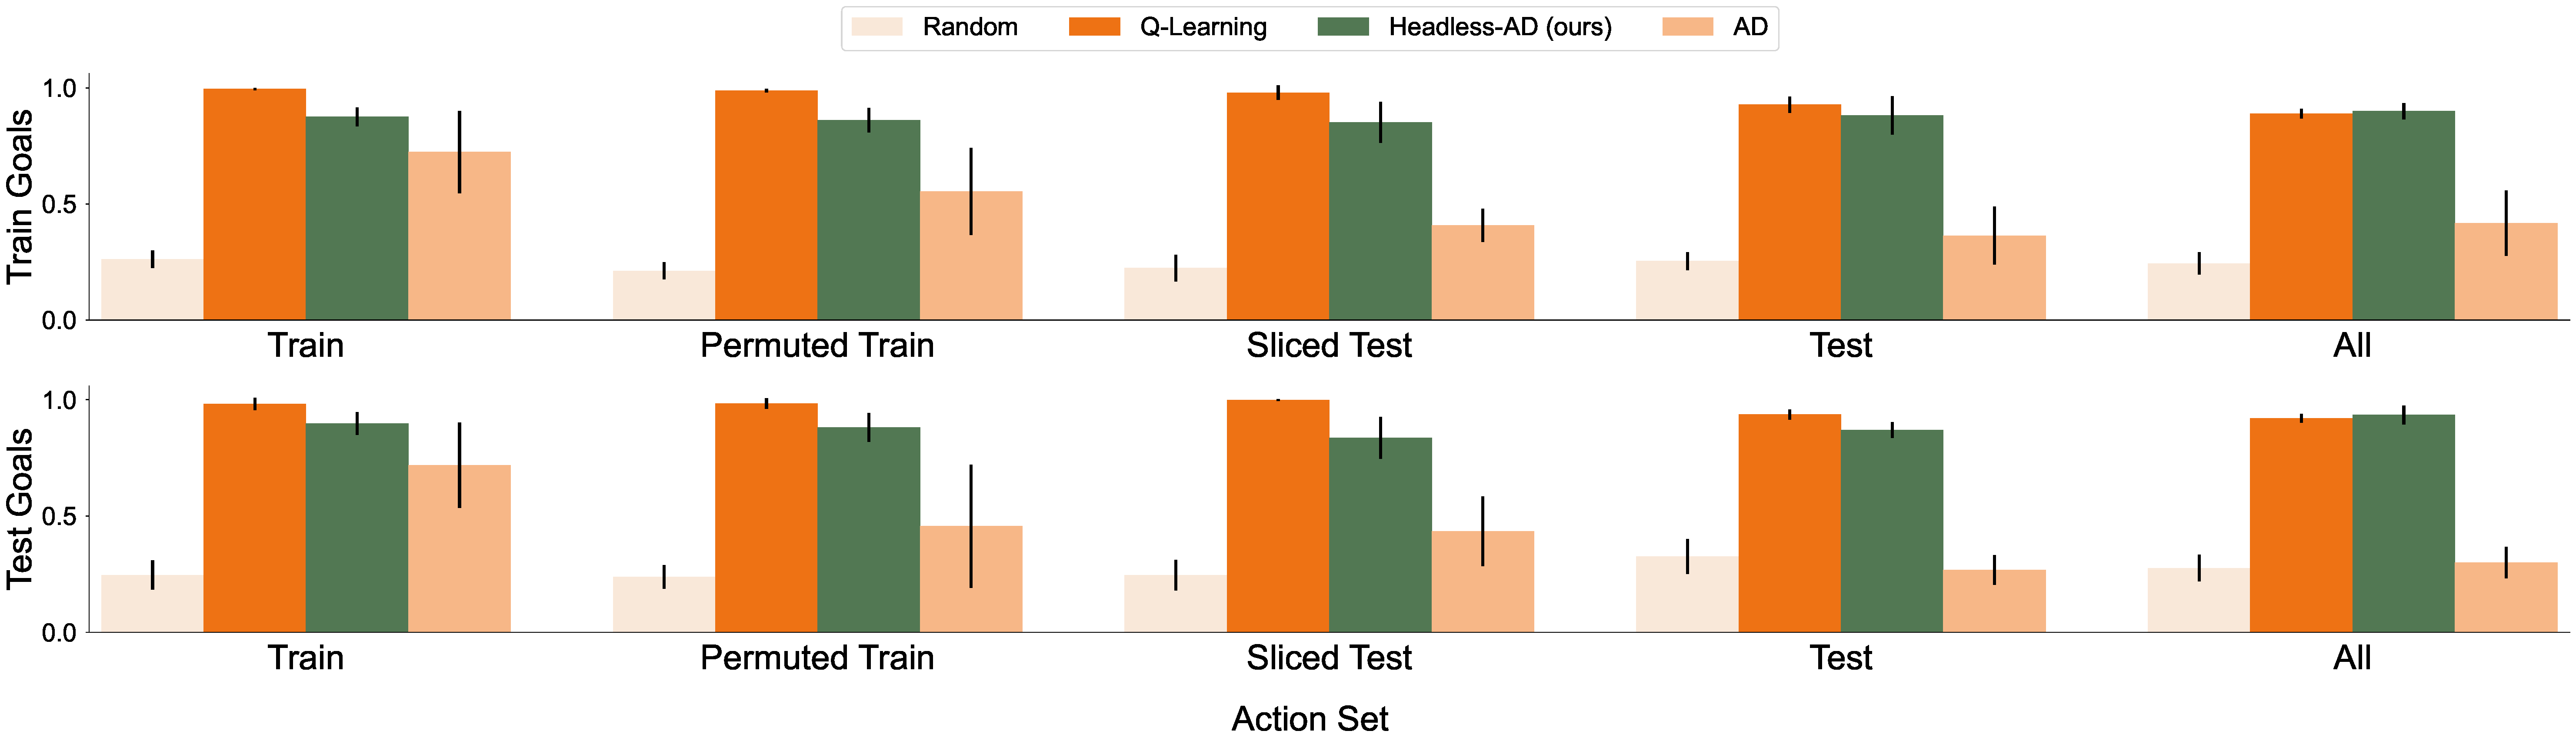
\includegraphics[width=0.9\textwidth]{images/visual_gridworld_bars.pdf}
    \caption{\textbf{Visual Darkroom:} Darkroom environment was modified to emit visual observations. Headless-AD consistently outperforms AD in this more complex observational setting.}
    \label{fig:visual_gridworld_bars}
    \vskip -0.2in
\end{figure*}